\documentclass[journal]{IEEEtran}

\usepackage{url}
\hyphenation{op-tical net-works semi-conduc-tor}


\usepackage{graphicx}
\graphicspath{ {./} }

\newcommand{\tx}[1]{\textsf{#1}}

\begin{document}
\title{Wolk Protocols for\\ Decentralized Web Applications}
\author{Sourabh Niyogi, Michael Chung, Alina Chu, Xinzhuo Han, \\
Tapas Jana, Mayumi Matsumoto, Anand Ray, and Rodney Witcher}

\maketitle

% As a general rule, do not put math, special symbols or citations
% in the abstract or keywords.
\begin{abstract}
Todays web applications operate in a paradigm of centralized servers exerting asymmetric control over  data silos.  We outline Wolk protocols for decentralized web applications that aim to reduce centralization by having user data, application data and shared blockchain state and indexes stored in blockchain.  We highlight aspects of our design and how to shift the balance of power from developers and platform owners to users.
\end{abstract}

\begin{IEEEkeywords}
decentralized storage, provable NoSQL, blockchain, cryptocurrency.
\end{IEEEkeywords}

\IEEEpeerreviewmaketitle

\section{Introduction}
\IEEEPARstart{C}{urrently}, web sites/applications are served under a domain by a web server who controls the web server.  Over the last 30 years, numerous centralized services have increasingly absorbed user data into silos, exerting centralized control over their users data with free(mium) business models coupled with Terms of Service that confer them rights.  When platforms are created to support access to this user data, the platform owner has reliably exerted paternalistic control over how this user data can be used, usually to preserve the platform owners status over their acquired users in predictably self-interested way.  Remarkably, the modern world has handed a handful of of these centralized web services powers of the same order of magnitude as nation-states, demanding new architectures that properly shift powers so users are not as helpless.  Many different kinds of efforts to decentralize all things exist, but our goal is to transfer power from platforms and developers to users in decentralized web services specifically.

Distributed ledger technologies may offer solutions to decentralizing who can control the next state of decentralized web applications to shift this power.  Nakamoto's Bitcoin showed that distributed ledgers secured with proof-of-work can be used in decentralized payment networks.  Ethereum and many other derivative blockchains demonstrated a much richer state space where "smart contracts" could flexibly compute state transitions of user data.  These next generation blockchains have operations powering some purported ``decentralized applications" (dapps). However, in the vast majority of cases, data and application code are still kept off-chain and solely rely on "trusted" oracle to supply the data feed, as the cost of running true dapps remains financially prohibitive.

A number of decentralized permissionless storage systems do not involve distributed ledger technology, and offer storage services at zero cost without a peer-to-peer.  Some systems, following in the model of BitTorrent, have user and developer data stored by actual user nodes in peer-to-peer network (c.f. DAT, GunDB) -- when requests are made to the network, responses are returned by a peer-to-peer network that store many copies of a particular users data where security is apparently demonstrated with redundancy but not provably so, with low concern for malicious actors.  Other systems focus solely on providing users control over their data through permissioning mechanisms (c.f Berners-Lee et al's SOLID, Blockstack's Gaia), with users trusting a pod provider or cloud storage if not hosting themselves.  These systems are in nascent development and will certainly evolve to parallel many centralized services (e.g. dTube matching YouTube), yet the economic model of these systems is ``pay Google Drive/Amazon S3/.. to keep your data''.  Oddly, proponents of these architecture purport that decentralization is achieved with physical and informational control over a USB stick or S3 account!

Systems of IPFS \cite{filecoin} and SWARM \cite{swarm}, following Sia \cite{sia}, and STORJ \cite{storj} actively tie cryptocurrency rewards to file storage and retrieval, backed by a Filecoin blockchain and Ethereum's Smart contracts.  We will be able to compare our systems to Filecoin and SWARM as our implementations are complete, but we have been pursuing an approach not using Kademlia-like DHTs, which have non-performant read performance.

As goal is to shift control from developers and platforms to users, we must make it clear that our meaning of the word ``decentralized" is: ``control is possible by many parties" and permissionless means ``any party can assume control".  If Bob keeps his data in numerous places with the help of Alice, he hasn't decentralized control: many cloud providers do this quite efficiently already.  If Bob uses a blockchain with a smart contract solely controlled by Alice, he hasn't decentralized control either: there is just a blockchain in front of a centralized service run by Alice.  If Bob uses a web site controlled by solely Alice at xyz.com that connects to a blockchain, there is just a centralized service run by Alice.  We believe users of decentralized web architectures deserve less decentralized snake oil.

\section{Design Overview}

Fundamentally our goal is design protocols for decentralized web applications to replace the centralized services in full, with users taking back control from developers via the following design:
\begin{itemize}
\item {\bf Users.} Users have Javascript browser clients holding private keys to interact with one or more Wolk storage nodes, receiving signed blockchain transactions with HTTP PUT/POST/DELETE to modify the state of the blockchain.  Figure~\ref{fig:transactiontypes} shows the list of transaction types.   When users create an account with \tx{SetName}, storage nodes sign up for the responsibility with \tx{ SetStorageClaim};  Users create and delete collections with \tx{ SetBucket} transactions and insert, update and delete key-value pairs with \tx{ SetKey}.  HTTP operations involve submitting public keys in JSON WebKey headers in all PUT/POST/DELETE/GET interactions between users and storage nodes.

\item {\bf Developers.}  Developers are simply users that store application code in their collections.  Application code written by developers use a wolk.js API to submit blockchain transactions using the WebCrypto API for key generation and signing on P-256 curves.   Several reference applications have been built in this way, shown in Figure~\ref{fig:applications}.  Users navigate to these applications by accessing {\em any} wolk node at: {\tt https://storagenodedomain/rodney/videos}.  Because the application code and user data is not controlled by the operator of the \tx{storagenodedomain}, and because the application can only write in prescribed ways to the user bucket with the wolk.js API, there is little opportunity for data silos to form.

\item {\bf Storage/Consensus Nodes.} Storage node operators operate Kubernetes clusters with Ceph \cite{Weil:2006:CSH:1298455.1298485} or similar high performance distributed storage, set up with Rook and referencing Wolk Docker containers for storage and consensus binaries.   The Storage node and Consensus node respond to user queries to evolve blockchain state to serve the users, using storage primitives of provable data storage (Section~\ref{sec:provabledatastorage}) and Algorand (Section~\ref{sec:blockchainconsensus}).   Storage nodes  register on the Wolk blockchain with \tx{RegisterNode} transactions that update a RegistryStorage SMT.   Every position in this node registry specifies a pair of storage and consensus service endpoints, where the pair shares the same Ceph local storage backend in Kubernetes.  At a given block, the registry $R$ is fixed but may evolve as users create new accounts.

\item {\bf Verifier+Liquidator Nodes.}  If computational resources allow, verifier nodes can also verify the state of user buckets by issuing deterministic random challenge to responsible storage nodes asking Replication Proof of User's data. Verifier nodes submit attestations to be included in proposals, where higher samples count and more frequent sampling increase the likelihood to be selected. Verifiers are held responsible for their committed work and audited by Liquidator nodes for fraudulent activity.

\end{itemize}
The Rewards protocol is reviewed in section~\ref{sec:rewards}.  It is not expected that mining rewards will be required long-term, however: the storage and bandwidth rewards are sufficient.

\begin{figure*}[h]
    \centering
\begin{small}
    \begin{tabular}{l|l|l}
    Category & Transaction Type & HTTP Operation \\ \hline \hline
      Node &   \textsf{RegisterNode(j int, ip string, port int, V int)} & PUT/POST/DELETE \\
           & \tx{SetStorageClaim(j int, owner string)} & PUT/POST/DELETE \\
           & \tx{GetNode(j int)} & GET \\  \hline
      Data Writes &   \tx{SetName(owner string})  & PUT/POST/DELETE \\
           & \tx{SetBucket(owner string, collection string)}  & PUT/POST/DELETE \\
           & \tx{SetKey(owner string, collection string, k string, v common.Hash)}  & PUT/POST/DELETE \\ \hline
       Data Reads  & \tx{GetName(owner string)}  & GET \\
       &  \tx{GetBuckets(owner string)}  & GET \\
       &  \tx{GetBucket(owner string, collection string)}  & GET\\
       &  \tx{GetKey(owner string, collection string, k string)}  & GET \\
       &  \tx{ScanCollection(owner string, collection string, start, end interface\{\})}  & GET \\
     \end{tabular}
\end{small}
    \caption{Wolk Writes are Signed Blockchain Transactions done with HTTP PUT/POST/DELETE operations; Reads are Signed HTTP GET operations.}
    \label{fig:transactiontypes}
\end{figure*}

\begin{figure*}[h]
\begin{scriptsize}
    \begin{tabular}{|l|l|} \hline
    (a) Block Explorer .                 & (b) Bucket Explorer \\ \hline
    \includegraphics[width=3in]{block_explorer.png} & \includegraphics[width=3in]{bucket_explorer.png} \\ \hline
    (c) NoSQL Explorer .                 & (d) Videos \\ \hline
    \includegraphics[width=3in]{nosql_explorer.png} & \includegraphics[width=3in]{videos.png}      \\ \hline
    \hline
     \end{tabular}
\end{scriptsize}
    \caption{Decentralized Web Applications work the same as web applications, but they are served from wolk blockchain nodes
    and write data to the blockchain rather than in centralized data silos.}
    \label{fig:applications}
\end{figure*}


\section{Primitives}

\subsection{Provable data storage}
\label{sec:provabledatastorage}

Two core data structures are used to support provable key-value pair data storage: SMT(Sparse Merkle Trees) and AVL(Adelson-Velsky and Landis) trees, with CRUD interfaces to insert, update, delete and get key-value pairs, plus AVL tree supporting ordered range scans.  Both data structures support provable key-value storage with Merkle branches that resolve to merkle roots committed in blockchain state.

\subsubsection{Sparse Merkle Trees}

The Sparse Merkle Tree \cite{Dahlberg2016EfficientSM,lauriekasper2012} abstractly represents a mapping between N-bit keys and M-bit values with $2^N$ leaves that Merkelize into a single Merkle root.  An empty tree has a empty value at all leaves, and at each of N levels there is a single default hash $d(i)$.  On each insert, a single leaf changes, but as almost all the $2^N$ leaves are the empty value, only the non-default values need to be represented closer to the root of the tree, with the SMT represented by  "chunks" by prefix tree.  In our implementation, all SMTs are 160-bits (20 bytes) or depth 160, where each byte of a key is used to traverse the tree 8-bits (nibble) at a time.  A particular SMT is referenced by a chunk hash, which is used as a key to find a chunk representing up to 256 children; each child can be an "internal" node with another 256 children or a terminal node.    Each child has an internal merkle root, chunk hash, a value hash, and a byte representing if it is terminal or intermediate node.   The internal merkle root caches the, supporting efficient recomputation of the SMT root.     Every \tx{Get} operation can return a proof of inclusion for the key, and well as a ``proof of exclusion" for when the value is the default value.   Figure~\ref{fig:smt} shows an SMT with two values $V_1$ and $V_2$ inserted by their respective hashes $H(V_1)$ and $H(V_2)$ -- the Merkle proof of inclusion for SMTs are generally compact with random keys because the majority of the values are default hashes.  So for example, the proof of inclusion for $H(V_1)$ only involves 1 hash and a single 160-bit stream marking which levels involve what non-default hashes.

\subsubsection{AVL Trees}

AVL Trees are binary search trees that compute balance factors at all times to ensure the tree is always balanced.  We adapted Tendermint's provable AVL representation to map into chunks (previously it was LevelDB-based) where each node in the AVL tree can have up to 256 children.  Now, when nodes in the tree become imbalanced, the tree is rebalanced to ensure that pairs of sub-trees in chunk space differ in height by at most 1.  Like the SMT, AVL trees are uniquely referenced by a chunk hash, but instead of traversing byte by byte, queries are by start and end range.

AVL Trees are used to provide range proofs on an indexed set of JSON documents.  Each range scan with $m$ results then can $m$ proofs of inclusion for each Merkle branches, resulting to the Merkle root of the AVL tree.  A user's collection, or a global collection can have multiple indexes.  An indexed collection of JSON documents has $N$ AVL trees for each of $N$ indexes in collection, where each index has a different chunk hash; adding a new element to the collection of documents involves $N$ updates.  To represent the evolving state of the collection requires a JSON record to aggregate the multiple indexes together.   For \tx{ScanCollection} operation to be possible on a collection, the collection must have an index on the attribute being ordered or filtered on.

\subsection{Blockchains and Consensus}
\label{sec:blockchainconsensus}

\subsubsection{Block Structure}

Each block packages an array of transactions and keeps a historical record of how these transactions effect evolving 4 state roots.  Here is the block structure:

\begin{footnotesize}
\begin{verbatim}
type Block struct {
    NetworkID     uint64
    ParentHash    common.Hash
    BlockNumber   uint64
    Seed          []byte
    NameRoot      common.Hash
    AccountRoot   common.Hash
    RegistryRoot  common.Hash
    KeyRoot       common.Hash
    Transactions  []*Transaction
    StorageBeta   uint64
    BandwidthBeta uint64
}
\end{verbatim}
\end{footnotesize}

The {\tt NetworkID} is used to support multiple chains at a time (e.g Testnet 1 ... 5), and the BlockNumber + ParentHash ; the Seed parameters are used in VRF based sortition.  The execution of transactions generally update one or more of the 4 state roots in each block:
\begin{itemize}
    \item Name Storage SMT - represents the mapping between user names and addresses, updated when SetName is applied.  Key: NameToHash(name) Value: Txhash of SetName.
    \item Account Storage SMT - represents the mapping between user names and Account objects, where Account objects hold balance, storage bytes used, quota, public key and the list of storage nodes who have committed:
\begin{footnotesize}
\begin{verbatim}
type Account struct {
    Address      common.Address
    Name         string
    Balance      uint64
    Quota        uint64
    Usage        uint64
    Nonce        uint64
    RSAPublicKey []byte
    StorageNodes []uint64
}
\end{verbatim}
\end{footnotesize}

    \item Key Storage SMT represents the mapping between various user names and collection names and the collection root hashes.
    \item Registry Storage SMT represents the list of storage nodes and the HTTP + P2P ports exposed so that other nodes can interact with them.  The Keys are the hash of the node position and the values are hashes of:
\begin{footnotesize}
\begin{verbatim}
type RegisteredNode struct {
    address     common.Address
    pubkey      *ecdsa.PublicKey
    valueInt    uint64
    valueExt    uint64
    storageip   string
    consensusip string
    region      byte
    httpPort    uint16
}
\end{verbatim}
\end{footnotesize}
\end{itemize}

\subsubsection{Transaction Structure}

We used {\tt go-ethereum}'s devp2p package for peer-to-peer and RLPx encoding for packaging  Transaction of the following form:

\begin{footnotesize}
\begin{verbatim}
type Transaction struct {
    Method  []byte
    Path    []byte
    Payload []byte
    Sig     []byte
    Signer  []byte
}
\end{verbatim}
\end{footnotesize}

\begin{itemize}
    \item {\tt Method} specifies one of "POST", "PUT", or "DELETE" with standard HTTP semantics.  We anticipate implementing "PATCH" in the future.
    \item {\tt Path} identifies the user, collection and key, depending on the Transaction Type:
    \begin{itemize}
        \item \tx{SetName} has owner, e.g. ``rodney"
        \item \tx{SetBucket} has owner + collection, e.g. ``rodney/videoobject"
        \item \tx{SetKey} has owner + collection + key, e.g. ``rodney/videoobject/gilroy.mp4"
        \item \tx{RegisterNode} has {\tt wolk/node/}{\em nodenumber}
    \end{itemize}
    \item {\tt Payload} specifies a JSON packet that depends on the Transaction Type.  Each of the Transaction Types in Figure~\ref{fig:transactiontypes} have a different payload structure:
    \item {\tt Signer} has the public JSON Web Key (P-256)
    \item {\tt Sig} is the Signing of the hash of concatenated Method, Path, Payload.
\end{itemize}

Transactions received by the guardian node are validated by matching the {\tt Sig} to the public key in {\tt Signer} prior to gossiping in the P2P network and included in the nodes transaction pool.



\subsubsection{Consensus Algorithm}

We implemented a consensus protocol similar to Algorand and eth2.0, which utilizes a leaderless proof-of-stake procedure to manage state transitions of the blockchain \cite{cryptoeprint:2018:377}. The consensus has nodes participating in committees in a multiple step process:
\begin{itemize}
    \item Proposal step.  If possible, nodes relay a proposal containing a list of transactions and an attestation along with a previous blockhash and a VRF proof.
    \item Reduction.  Nodes submit their votes on the highest priority proposal from the Proposal step.
    \item Soft vote.  Nodes soft vote for a single proposal in the previous reduction step.
    \item Cert vote.  Nodes cert vote for a single proposal from the previous soft vote step.
    \item Next vote.  Nodes next vote for a single proposal from the previous cert vote step.
\end{itemize}
All committee members may propose a block.  If the majority of nodes registered with stakes are honest, then if the committees are large enough, then the probability of  committees with majority of the committee members being dishonest can be kept low.

The overall shape of the consensus process has nodes going through a sortition process to generate proposals, where each node has a provable number of {\em votes} that is verifiable by other members in the committee as being correct.  Currently all committee members have fixed amount of stakes. Once the number of votes exceeds a {\em tentative} threshold, a node can advance from one step to the next, but only when the number of votes exceeds a {\em finalized} threshold can a node know for certain that there is no possibility of a fork. Our implementation is flexible and can be modified such that larger stakes support higher priority, the probability of being the highest proposal generated in the committee is proportional to the stake.


\subsection{Storage of User and Blockchain Data}
\label{sec:storage}

Storage nodes must redundantly encode user and blockchain data as transactions are applied; nodes must receive rewards for valid storage and penalties for losing storage, which we review in Section X.  There are several different kinds of data generated:

\begin{table*}[h]
 \begin{small}
    \begin{tabular}{l|l|l}
      Data Kind        & Held by & Example \\ \hline
      User Data (Files, Records)        & storage nodes who submit \tx{SetStorageClaim} & /rodney/videoobject/gilroy.mp4 \\
      User Indexes (SMTs, AVLs)   & storage nodes who submit \tx{SetStorageClaim} & /rodney/videoobject/commentCount \\
      Blockchain Data (Blocks, Txs)  & committee members who vote on a block          & /wolk/block/42 \\
      Shared Blockchain Indexes (SMTs, AVLs)  & committee members who update the index         & /wolk/videoobject/commentCount \\
    \end{tabular}
    \caption{Kinds of Data}
    \label{tab:datatypes}
 \end{small}
\end{table*}

\begin{figure}
    \centering
    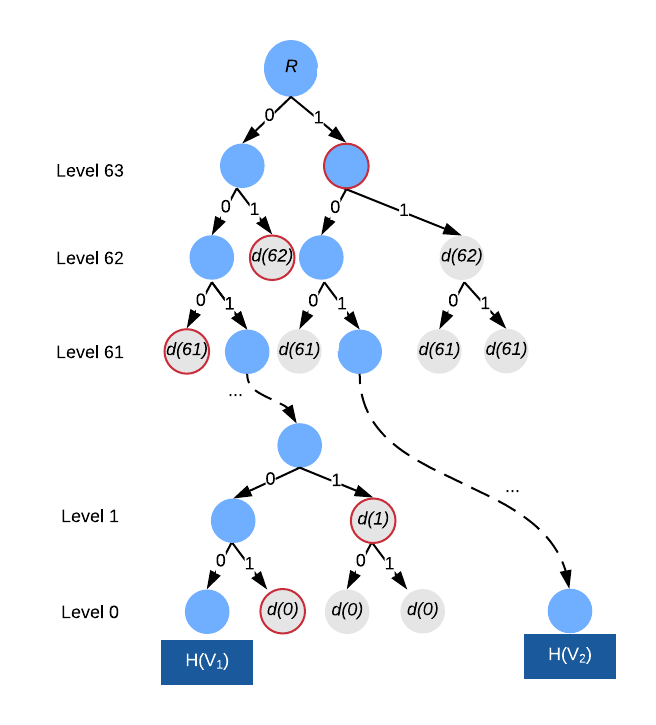
\includegraphics[width=3in]{SMT.png}
    \caption{160-bit Sparse Merkle Tree.}
    \label{fig:smt}
\end{figure}

For proof of replication, we are currently using Pietzrak (2019)'s Depth Robust Graph (DRG) encoding scheme \cite{pietrzak:LIPIcs:2018:10152} which has each users data appended to an append-only log (see also Fisch (2018) \cite{cryptoeprint:2018:678} used in Filecoin, which also uses DRG).  A simplified version is shown in Figure~\ref{fig:proof-of-replication}.  The key property of the encoding scheme is that the users data is encoded with the DRG in such a way that a storage node cannot decode the data and provide proofs of replication quickly unless it is actually storing the encoded data.  We situate this scheme for user data and user indexes in the following way:

\begin{enumerate}
\item User $U$ posts a new record $F$ to guardian node $G$ along with a signed transaction including $H(F)$, the hash of $F$.

\item Guardian node $G$ notifies storage nodes $x_1 \ldots x_N$ responsible for storing $U$'s data.

\item Storage nodes request raw $F$ from $G$.

\item During the execution of block $B_i$, storage nodes are notified by $B_i$'s committee that User Index chunks are available.

\item Storage nodes responsible for $U$'s data request raw index chunks $I$ from the committee.

\item Immediately after each block $B_i$ is finalized, storage nodes responsible for user $U$ append new raw user data $F$ and user index $\cal{I}$.

\item Each storage node $x$ is responsible for different users $U_1 \ldots U_{num(x)}$, which each have different encodings of the user data and user indexes.   Every epoch, storage node $x$ broadcasts a single meta Merkle root $M_x(y)$ representing all the users the storage node $x$ is encoding data for, ordered by user address.

\item A verifier $V$ keeps the committed meta Merkle roots in memory and uses a VRF-based scheme to query a specific user $U^*$ at a specific byte $b$ -- all the storage nodes storing $U^*$ are queried for a Merkle branch that must resolve to the committed merkle root, and the merkle root must also resolve to the meta merkle root broadcasted.  We review this process in Section~\ref{sec:verifierliquidator}.
\end{enumerate}

\begin{figure}
    \centering
    \includegraphics[width=2.5in]{ProofOfReplication.png}
    \caption{Adapted from Pietrzak (2019)'s toy example of a depth robust DAG  $G = (V, E), V = \{1, \ldots , 6\}$ with $VC = \{3, . . . , 6\}$ being the challenge nodes. The embedded data is shown in blue, the labels the prover stores are in red.}
    \label{fig:proof-of-replication}
\end{figure}

Whereas user data and user indexes are held by storage nodes who commit to storing particular users, blockchain data and shared blockchain indexes are held by committee members.  This approach departs from earlier designs of many decentralized storage systems that use the chunk hashes to index into a distributed hash table held by a peer-to-peer network; in practice, p2p networks (e.g. Filecoin and SWARM) are fatally slow and require the reader to wait a long time to know if a chunk is not available.  Instead of using the what as a key (a file or chunk hash) resulting in a $O(\log n)$ lookup, the approach is made $O(1)$ using the who as key (for user data) and when (for blockchain data), resulting in a more performant read model:
\begin{itemize}
    \item {\em User data}.  When reading data concerning a user $U$ (e.g. \tx{rodney/videoobject/gilroy.mp4}), read the storage nodes responsible for storing $U$ (e.g. nodes 14, 17, 241, 293) in the account storage SMT.  Query those storage nodes, who will have the raw user data and indexes.
    \item {\em Blockchain data}.  When reading data concerning a global index relative to the latest block, the committee is known.  Query the committee, who will have the blockchain data and indexes.
\end{itemize}

Each request of the guardian $G$ can result in a query by the guardian to do parallel reads (querying all the storage nodes responsible for a user, or all the members in a committee) or in serial fashion (querying the one node or member apparently closest to the querier) until a result that can be returned.  If the responder can provide a proof of replication for the user data being specifically queried quickly, then the guardian could  redirect the request to the first responder who actually does so.  Otherwise, the guardian will typically act as a proxy server.


\subsection{Verifier and Liquidator Roles}
\label{sec:verifierliquidator}

Verifiers periodically initiate Proof-of-Replication Challenges and package $k$ verifiably-random sequential challenges into an {\tt Attestation}:

\begin{footnotesize}
\begin{verbatim}
type Attestation struct {
    BlockHash    common.Hash // Attested BlockHash
    BlockNum     uint64      // Attested BN
    MaxVPriority *VPriority  // VPriority
    Signature    []byte      // Verifier Sigs
}
\end{verbatim}
\end{footnotesize}

A valid Attestation must contain a non-empty VPriority matching to Verifier's Signature:

\begin{footnotesize}
\begin{verbatim}

type VPriority struct {
    KSeed    []byte // Input msg used to generate VRF
    Verifier []byte // Verifier's pubkey
    VRFProof []byte // Verifier's Proof
    MaxPrior []byte // MaxPrior given k sub-unit
    K        uint32 // Security level
}

\end{verbatim}
\end{footnotesize}

Per each Attestation, Verifiers use $KSeed$ (derived from attested block) to generate their own $VRFProof$ and issue sequential challenges using $priorityHash$:

\begin{footnotesize}
\begin{verbatim}
   KSeed2VRFProof(privKey, Kseed) = VRFproof
   priorityHash(vrf, j) = hash(vrf,j)
   sampleFromVRF(vrf, j) = (user, challengeIdx)
\end{verbatim}
\end{footnotesize}

At high level, Account SMT contains all users of the network, with leaves nodes holding an Account structure maintaining a Quota and actual Usage. Verifiers compute   $priorityHash(vrf,j)$ from $VRFProof$ for $j \in (0,k;j$++$)$ and sample Account SMT $k$ times before allotted period $T_{Allotted=15sec}$ is completed.

Each of the $priorityHash(vrf,j)$ within $k$ sample are mapped into a deterministic random byte in the Account SMT, which results in a Proof-of-Replication challenge sent to all the responsible Storers selected by the algorithm. Responsible Storers must respond with a complete Merkle branch proof matching to its previously committed root within $T_{Replication=10sec}$.

A signed Attestation is then broadcasted to the Network. Consensus Node select the best Attestation to be included in its proposal, determined by the the score:
\newline $Score_{A}$ = $max(VPriority) \cdot \frac{K_{eq}}{ (BN_{Proposed}- BN_{Attested})}$, where
\newline $max(VPriority) = max(priorH(VRF,j),j \in (0;k; j))$. The algorithm has some desirable properties: (a) newer Attestation is preferred over older ones (b) Verifier's Priority is deterministic random and derived challenges are sequential, therefore resistant to Sybil attack by construction.


\subsection{Node Replacement and Registry Mitosis}
\label{sec:nodedynamics}

We desire that node $y$ be able to replace node $x$ in a registry $R$ in timescales on the order of a day, and not depend solely on $x$ to do so.
Having high replication levels ($> 3$) for user data and committee sizes being large (or entanglement codes \cite{DBLP:journals/corr/abs-1810-02974}) support $y$'s ability to replace $x$ reliably without $x$'s existence.
To ensure this is possible, on average, we require that $x$ be limited to ensure than no more than a certain amount of data be encoded.
Here are the encoding times for 3 tiers of service, which imply that a \tx{SetStorageClaim} transaction for node $x$ must be rejected if $x$ is committing to a Quota that exceeds 10TB in aggregate:

\begin{table}[]
    \centering
\begin{tabular}{l|l|l} \hline
 Size   & Min.  Node Startup Time/Cost & Tier Maximum \\ \hline
  100G  & 1000s	= 16.6min  & Tier 0 Max \\
  1TB   & 10000s = 2.7hr   & Tier 1 Max \\
  10TB  & 100000s	= 27hr & Tier 2 Max \\ \hline
\end{tabular}
    \caption{Encoding Times for User data}
    \label{tab:my_label}
\end{table}

If node $x$ has committed to a single Tier 2 user or 10 Tier 1 users or 100 Tier 0 users, then $x$ cannot be allowed to accept any new users, because otherwise the time to replace $x$ would exceed one day.

With the above constraint limiting nodes to a certain Quota maximum individually, the aggregate quota maximum across all nodes in the registry can be used to trigger registry mitosis, wherein the registry size doubles in a block if the result of 1 or more account creation (`SetName`) operations will exceed the Quota Max as listed in Table~\ref{tab:registrygrowth}.

\begin{table}[]
    \centering
\begin{tabular}{r|r} \hline
Registry     & Quota Max \\ \hline
8            & 64TB   \\
16           & 128TB  \\
32           & 256TB  \\
64           & 512TB  \\
128          & 1PB    \\
256          & 2PB    \\
512          & 4PB    \\
1,024        & 8PB    \\
2,048        & 16PB   \\
4,096        & 32PB   \\
8,192        & 64PB   \\
16,384       & 128PB  \\
32,758       & 256PB  \\
\end{tabular}
    \caption{Registry and Max Quota}
    \label{tab:registrygrowth}
\end{table}

On such a mitosis event, every node $x$ in a $2^q$-sized registry is copied into $x_1$ and $x_2$ in a $2^{q+1}$-sized registry.  Accounts are split into the even or odd node based on the least significant bit of account addresses being stored at the mother node.
That is, if representing 1PB is possible for 128 nodes, growing by a factor of 128 to 16PB would be expected to have 7 mitosis events with 16384 node positions, with each node carrying the same average load.
After this level of growth, the viewpoint of node $y$ replacing some node $x$ in one of those 16384 node positions would be same as before those 7 mitosis events.  We leave the design question of how to support users with storage plans greater than 10TB aside for now.

\subsection{Application Data Model for Trustless App Stores}
\label{sec:jsonld}

Decentralized web applications demand that public collections support multiple applications which read and write user data in prescribed ways.  Web applications should never hold user data in developer collections in the current way centralized servers do.   Instead, applications should record user data in user buckets and global public indexes.   An application developer should typically build solely with the default schemas.  We achieve {\em developer replacability} by having user collections and global indexes conform to standardized JSON-LD schemas (specified by schema.org) and replicated in global blockchain \tx{wolk} indexes.   There are different kinds of collections:
\begin{itemize}
    \item {\em Shared} blockchain indexes are held by the committee members who update the index in each block.  This index indexes the metadata of user content.
    \item {\em User} indexes, held by the storage nodes for the user.   User index contain all data referred to by the shared blockchain indexes.  Anytime a global collection is updated, raw data in the standard collection is first updated.  It then applies the metadata to the user collection and then to the Global collection.
    \item {\em User data} collections, held by the storage nodes for the user.
\end{itemize}


\begin{figure}
\begin{scriptsize}
\begin{verbatim}
{
  "@type": "VideoObject",
  "identifier": "heather/VideoObject/gilroy.mp4",
  "description":"News coverage of Gilroy Garlic festival",
  "contentUrl":"wolk://heather/VideoObject/gilroy.mp4",
  "thumbnailUrl":"wolk://heather/ImageObject/gilroythumb.jpg",
  "duration":"PT4M5S",
  "encodingFormat":"video/mpeg",
  "uploadDate": "2019-08-08T15:55:00"
  "author":"wolk://heather",
  "keywords":"gilroy, california, news",
  ...
}

{
  "@type": "WebApplication",
  "identifier": "rodney/music",
  "author":"wolk://rodney",
  "creator":"wolk://rodney",
  "name":"Music App",
  "description":"Organizing the world's music!",
  "thumbnailUrl":"wolk://rodney/ImageObject/musicicon.png",
  "version":"3.0",
  "keywords":"music songs instruments",
  "installUrl": "wolk://rodney/music/install.html",
  "contentLocation":"wolk://rodney/music/",
  "genre":"Entertainment",
  "requiredCollections":["AudioObject","Action","ImageObject"]
}

{
  "@type": "LikeAction",
  "id": "412",
  "agent": "sourabh",
  "object": "rodney/webapplication/music"
}
\end{verbatim}
\end{scriptsize}
\caption{\label{fig:jsonld} Sample JSON-LD records}
\end{figure}

The JSON-LD model pioneered by schema.org is powerful enough to represent socially linked data such as "sourabh likes Rodney's Music application".  However, because schema.org does not make it clear which attributes are required vs optional or indexed, the intention of representing {\tt .jsonld} in the \tx{wolk/schema} collection attempts to documents the increased structure imposed in application data.   Given these recorded schemas, a Wolk node will be expected to keep a ontology of ``is a kind of" relationships for validation in SetKey transactions, e.g. that a certain input is a valid in having a certain type of \tx{object} ( \tx{InstallAction} should  have an \tx{object} of type \tx{WebApplication} that is valid and exists, \tx{BefriendAction} should have an \tx{object} of type \tx{Person} that is valid and exists, and so on.  To illustrate, here are schemas we are working with:
\begin{itemize}
    \item CreativeWork: VideoObject, WebApplication
    \item Action:  LikeAction, DislikeAction, CommmentAction, InstallAction
\end{itemize}
with sample JSON records for a \tx{VideoObject},  \tx{WebApplication} and \tx{LikeAction} shown in Figure~\ref{fig:jsonld}.


Much of the data of today's social applications can be trivially represented in the JSON-LD model, with ``Action" being performed on some derivate of ``CreativeWork", and social applications being then interchangable with one another.  We have developed multiple applications that use the wolk.js to submit transactions and do read queries with the chain:
\begin{itemize}
    \item Block Explorer
    \item Bucket Explorer
    \item NoSQL Explorer
    \item Videos
\end{itemize}
Screenshots for the above are shown in Figure~\ref{fig:applications}.  Critically, if another application developer cloned the code and offered completely different styled application to interact with the Videos, the underlying data storage would not change.  Because the developer does not write the user data into a silo locked behind a centralized server behind xyz.com, the developer cannot lock in the user.  Instead, if xyz app goes down, any number of similar services on an appstore can take its place.


\subsection{Decentralized Indexes}
\label{sec:sideeffects}

Many decentralized applications are made social with multiple users writing to shared  global indexes.  Using these shared global indexes, basic ranked results can be returned.  In our first few applications, we have implemented ``side-effect" rules to support these ranked results to match some of the commonly found features of Facebook and YouTube.   When users submit \tx{SetKey} transactions in the global {\tt action} index, this triggers updates to another index depending on the kind of action taken:

\begin{itemize}
    \item A {\tt CommentAction} will trigger an increment of the {\tt commentCount} on the {\tt object} referenced in {\tt CommentAction}
    \item A {\tt LikeAction} will trigger an increment of the {\tt upvoteCount} on the {\tt object} referenced in {\tt LikeAction}
    \item A {\tt InstallAction} will trigger an increment of the {\tt installCount} on the {\tt object} referenced in {\tt InstallAction}
\end{itemize}

A \tx{ScanCollection} operation on the global index on the most commented on, most liked, most installed etc. application can be returned accordingly.

\section{Storage Node Economics}
\label{sec:rewards}

The blockchain accepts paid transactions for new nodes joining the registry $R$ at position $j$ out of $2^q$ nodes using a \tx{RegisterNode} transaction.  With the analogy of {\em node position are land}, we adapt Posner and Weyl's Radical Markets \cite{radicalmarkets} ``self-assessment'' / Harberger taxes model where owners regularly self-assess the value of their node at $V_{int}$.  Alternate owners may freely acquire node $n_i$ by paying $V(n_i)$ in a  $\tx{Register}$ transaction composed of both:
\[
    V(n_i) = V_{int}(n_i) + V_{ext}(n_i)
\]
That is, nodes join by paying \tx{V} (matching $V(n_j)$ see below) in a signed \tx{RegisterNode} transaction, and may update the node at any time with a signed \tx{UpdateNode} transaction.

The underlying assumptions here:
\begin{enumerate}
    \item the current owner to pay taxes and assess the value $V_{int}(n_i)$ honestly
    \item the current owner of $n_i$ will, in order to prevent a node takeover, will be responsive to requests over a long period.  If non-responsiveness is an issue, $V_{ext}(n_i)$ will  be reduced so  new entrants are incentivized to see replacing the node as increasingly economically viable \item a potential new owner is willing to pay $V(n_i)$  based on the income it generates.
    \item an honest block proposer honestly adjusts evaluation $V_{ext}(n_i)$  upwards (or downwards) when it succeeds (or fails) to verify submitted storage claims by $n_i$.
\end{enumerate}
Taxes are deducted by the block proposer from its own balance based on:
\begin{enumerate}
    \item when the node was acquired through a \tx{Register} transaction
    \item when the last block was paid
    \item the taxation rate $\gamma$
\end{enumerate}

Storage nodes are incentivized to:
\begin{itemize}
    \item earn storage rewards by store replicas of user data and user indexes by fetching user data from guardian nodes and fetching user indexes from committee members
    \item earn mining rewards by storing blockchain data by participating in consensus committees
    \item earn bandwidth rewards by responding to GET queries
    \item maintain a good node valuation, and report valuations of itself when proposing blocks
\end{itemize}

It is not the case that a single storage/retrieval failure slashes a nodes stake -- instead, nodes that fail to user and blockchain data gradually have their node valuation reduced, with reduced valuations corrected with consistent uptime.

\subsection{Storage Rewards}

Any node $n_i$ in $R$ may submit {\em storage claim} transactions to the blockchain to earn Wolk tokens for storing chunk replicas in the following way:
\begin{itemize}
    \item Nodes in the blockchain use the signature $\sigma(B_j)$ of the previous block $B_j$ to select $c$ chunks {\em close} to the signature and submits $\tx{SubmitStorageClaim}(j, \sigma(B_j), c, R(c), \sigma)$ transactions for some chunk $c$ having a replica $R(c)$ held by $n_i$.
    \item A block proposal containing these storage claim transactions must submit the {\em oldest} $M$ valid storage claims in its block; a claim is valid if the chunk $c$ can be built from the neighborhood of nodes responsible for $c$.  For each valid claim, a balance will transfer from the chunk owner $\alpha(sizeof(c))$ to the node making the claim, using a pricing $\beta_s$.  Nodes will not submit storage claims with zero-balance accounts as they would have no effect, and may remove chunks so detected as a form of garbage collection.   The rationale of choosing the {\em oldest} chunks for inclusion and those chunks being close to $\sigma(B_j)$ is to limit the possibility that nodes will simply store a small number of test chunks; the earliest chunks are preferred because they are the least likely to be cached.
    \item As nodes succeed (or fail) to respond in time to requests for a replica of a chunk in the above validation process, the block proposer will adjust the blockchain's external valuation of the node $V_{ext}$ higher (or lower) by $\Delta_{+}$ (or $\Delta_{-}$:
    \[
    V_{ext}(n_i) = \left\{
    \begin{array}{ll}
    \max(V_{ext}(n_i) + \Delta_{+}, V_{int}(n_i)) & \mbox{on success} \\
    \min(V_{ext}(n_i) - \Delta_{-}, -V_{int}(n_i)) & \mbox{on fail}
    \end{array}
    \right.
    \]
\end{itemize}

\subsection{Bandwidth Rewards}

Nodes responding to \tx{Get} requests from users and peers tally how much bandwidth has been used by the requester without a corresponding payment.  If critical threshold $T_{payat}$ is reached, the node may halt responding until a signed ``check'' is relayed that brings the balance down to approximately zero.   The node can then submit signed checks to the Wolk Cloudstore blockchain with a \tx{SubmitBandwidthCheck(signedchecks []common.Check)} transaction, which will cause cryptocurrency tokens to be transferred from all the peers and users that wrote signed checks to the submitter (assuming signatures are valid, with positive balances).

\subsection{Mining Rewards}

Mining rewards of 20MM WOLK will be allocated to miners in the first 10MM blocks (est 3 yrs) in accordance with the simple schedule shown in Table~\ref{tab:mining}.  It is expected that a sharding model with each shard having its own chain will be developed by this time.

\subsection{Storage and Bandwidth Pricing}

To enable nodes to adjust the pricing of bandwidth to market conditions, each node also submits in its block proposal:
\begin{itemize}
    \item the amount of bytes of storage $\beta_{s}$ it believes should be represented by 1 Wolk token; the value may be adjusted upwards or downwards by not more than 1\%
    \item the amount of bytes of bandwidth $\beta_{b}$ it believes should be represented by 1 Wolk token; ; the value may be adjusted upwards or downwards by not more than 1\%
    \item the internal valuation of the node $n_i$ on itself $V_{int}(n_i)$
    \item the taxation rate $\gamma$; this value may be adjusted either direction by up to 1\%, subject to boundary conditions of $0 \le \gamma \le 1$
\end{itemize}

\begin{table}[h]
    \centering
    \begin{tabular}{|l|l|l|} \hline
        {\bf Block Number}      & {\bf Mining Rewards}    & {\bf Total Rewards} \\ \hline
        2          - 5,000,000  &  2.0 WOLK / block & 10.0MM WOLK [1.5yrs] \\
        5,000,0001 -10,000,000  &  1.0 WOLK / block & 5.0MM WOLK [1.5yrs] \\
        \hline
    \end{tabular}
    \caption{Mining Rewards}
    \label{tab:mining}
\end{table}

\section{Implementation and Performance Testing}

We implemented the Wolk node in Golang, available at {\tt https://github.com/wolkdb/cloudstore}.  Wolk binaries are compiled into Docker containers and uploaded to a public Google Container Registry.    We have deployed 8 to 128 node clusters in Kubernetes in Google Cloud, AWS, Azure, and Alibaba in the configuration shown in Figure~\ref{fig:kubernetes}(a).   Each storage / consensus node IP/Port information is initially registered in the genesis block for the initial 8 nodes.

\begin{figure}
    \centering
    \begin{tabular}{c}
     (a) Service / Deployment Model \\
     \includegraphics[width=3.5in]{kubernetes.png} \\
     (b) Multiple Cloud Provider Test Configuration  \\
     \includegraphics[width=2.5in]{federated.png}
    \end{tabular}
    \caption{Kubernetes Deployment}
    \label{fig:kubernetes}
\end{figure}

For latency and throughput testing, we use a {\tt wolkbench} utility supports submitting a consistent throughput of {\tt SetKey} transactions for files of a particular size (e.g. 10K, 1MB, or 10MB) or records for a certain number of accounts and collections after an initial set up period.

All our tests thus far have been with one cloud provider with 8-16 nodes spread out in 2-4 different regions; for cost-effective testing, we expect to have 8 Kubernetes clusters in 8 different regions, as depicted in Figure~\ref{fig:kubernetes}(b).  We are implementing the registry mitosis, verification and liquidator processes and explorer Kubernetes' federated architecture.  We expect to report on latency and throughput at peak volumes by the end of this year.

\section{Conclusions and Future Work}

In Wolk's architecture, user data, shared indexes and application are not held under the control of developers, but instead by interchangeable Wolk storage nodes who participate in decentralized consensus protocols.   We demonstrated that it is possible to combine decentralized storage with new consensus algorithms to have usable decentralized applications.

Developers who are accustomed to hosting their application code and ``their" users data on developer-controlled servers will need to  acclimatize themselves with this new model where they do not have control over their data and work with users not from day 0.  Any ambition that data moats can be constructed will be thwarted.  On the other hand, there is no platform owner to thwart the developer's ability to serve users, because the Wolk protocol replaces the platform owner and its APIs on web completely.  Developers who have been fearful of Twitter or Facebook kicking them off their.  Unfortunately, for mobile applications, Apple and Google wield dictatorial platform control to their appstore.

Users must have decentralized web applications to behaving like their centralized counterparts in having performant read/write operations.  Needing 10+ seconds to fetch a piece of content was acceptable for large files from BitTorrent, but high throughput low-latency is an absolute requirement for modern users.  So we aim to have most user queries be preemptively executed on guardian nodes, where transactions without guaranteeing finality is necessary to yield responsive applications; in this conception, only a fraction of queries will require finalized blocks and proofs only requested in $<1\%$ of queries as a spot check.

Needless to say, our use of blockchain for write operations requires a different form of UI than offered by early dapps that demand user payment and/or user approval of every write (e.g. as Metamask is wont to do), which should be recognized as acceptable for payments but not decentralized web applications.

\bibliographystyle{unsrt}
\bibliography{main}

% use section* for acknowledgment
\section*{Acknowledgment}

The authors would like to thank Viktor Tron and the Ethereum SWARM team
for encouragement and technical discussions.
This work has been supported by contributions from
Wolk token holders.

\end{document}
